\section{Intersection Computation}

\label{section:isect}

In this step, the intersections between faces are determined by triangle-triangle intersection tests. We use  M\"{o}ller's algorithm \cite{moller1997fast} because of its efficiency and simplicity. To ensure exact intersection computation, we integrate plane-based geometry into this algorithm. In the following, we first describe our space division algorithm, which reduces the number of intersection tests. Then our plane-based intersection algorithm is introduced. Lastly, we discuss how to deal with degenerate situations.

\subsection{Space Division}
\begin{wrapfigure}{r}[0in]{0in}
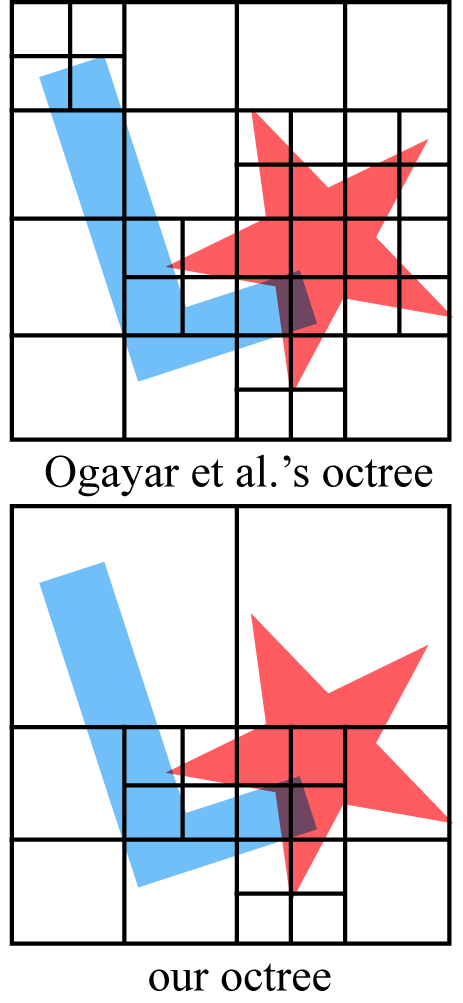
\includegraphics[width=1.2in]{boolean-10}
\end{wrapfigure}

As intersection detection is performed between each pair of faces, space division is necessary to reduce the number of testing pairs. We use an adaptive octree for this purpose. Our implementation is akin to the implementation of Ogayar et al. \cite{ogayar2015deferred}. The intersections between triangle faces and octree nodes are efficiently detected using the separating axis theorem \cite{gottschalk1996obbtree}. Octree leaves are classified into two types. If all faces that intersect a leaf belong to the same mesh, we regard it as a \emph{normal cell}. Otherwise, it is regarded as a \emph{critical cell}, within which the triangle-triangle intersection tests are performed.


The difference between our octree and that of Ogayar et al. is that we do not subdivide any normal cell, no matter how many faces it contains. Subdividing normal cells is only beneficial for the point-in-polyhedron test \cite{frisken2002simple}, which is seldom used in our method. This simplification saves significant computing time, especially when intersections between primitives are sparse located in small regions.

\subsection{Plane-Based Intersection Test}

We first make a quick review of M\"{o}ller's vertex-based algorithm. Then we introduce our implicit representations of intersections using planes. After that, we discuss how to implement M\"{o}ller's algorithm using plane-based geometry.

\subsubsection{Review of M\"{o}ller's algorithm}


\begin{figure}[t]
\centering
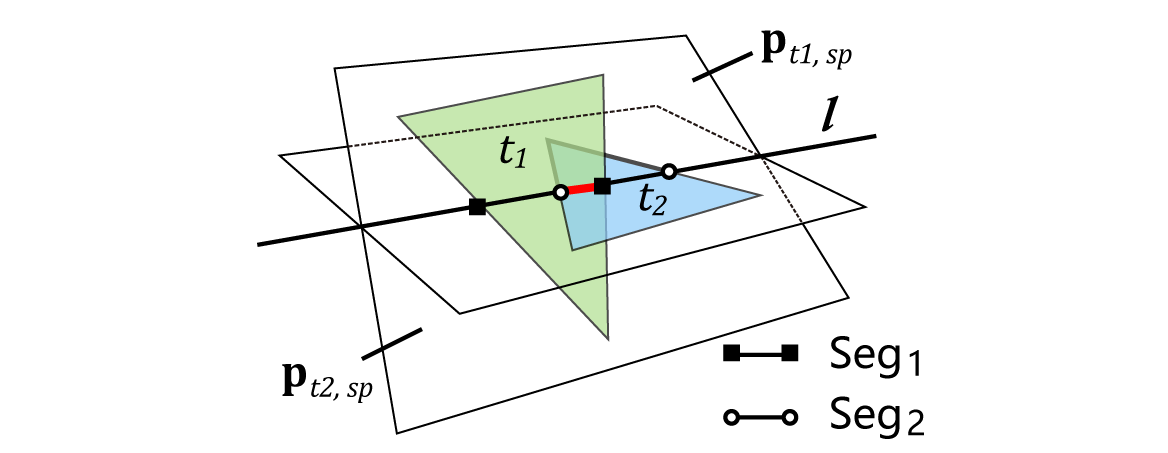
\includegraphics[width=3.5in]{boolean-12}
\caption{$Seg_1$ is the intersection between $\bm{p}_{t_2, sp}$ and $t_1$. $Seg_2$ is the intersection between $\bm{p}_{t_1, sp}$ and $t_2$. The intersection between $t_1$ and $t_2$ (red line segment) is the overlap of $Seg_1$ and $Seg_2$.}
%Seg1 is the intersection between pt2,sp and t1. Seg2 is the intersection between pt1,sp and t2. The intersection between t1 and t2 (yellow line segment) is the overlap of Seg1 and Seg2.
\label{fig_projection}
\end{figure}


M\"{o}ller's algorithm computes the intersection between two triangles $t_1$ and $t_2$ in three steps as shown in Fig. \ref{fig_projection}:
\begin{itemize}[leftmargin=0.45cm]
\item[1)] An early rejection is performed by testing whether $t_1$ intersects $\bm{p}_{t_2, sp}$, the supporting plane of $t_2$. The same test is also carried out between $t_2$ and $\bm{p}_{t_1, sp}$.
\item[2)]The intersection between $t_1$ and $\bm{p}_{t_2, sp}$, denoted as $Seg_1$, and the intersection between $t_2$ and $\bm{p}_{t_1, sp}$, denoted as $Seg_2$, are computed separately.
 \item[3)]The intersection between $t_1$ and $t_2$ is determined by computing the overlap between $Seg_1$ and $Seg_2$ .
\end{itemize}



The non-robustness of this algorithm stems from computing the coordinates of the intersection vertices (the end points of $Seg_1$ and $Seg_2$). Although implementation of this algorithm with arbitrary precision arithmetic produces exact coordinates, it is too costly for boolean evaluations with large CSGs.

\subsubsection{Plane-based intersection representation}
\label{sec:ir}

In our method, an intersection line segment  $\bm{\mathcal{I}}$ is stored as $\{T, \bm{P}_{ext}, \bm{P}_0, \bm{P}_1, \mathcal{N}\}$. This is the plane-based intersection representation (PBI-rep,  see Fig. \ref{fig:pbi}). The first component, $T$, indicates which triangle $\bm{\mathcal{I}}$ lies on.
$\bm{P}_{ext}$ indicates the plane that $\bm{\mathcal{I}}$ lies on. $T$ should not be in $\bm{P}_{ext}$. Thus the first two components indicate that  $\bm{\mathcal{I}}$ lies on the line $T \cap \bm{P}_{ext}$.
Then two end points of $\bm{\mathcal{I}}$ are $T \cap \bm{P}_{ext}\cap\bm{P}_0$ and $T \cap \bm{P}_{ext}\cap\bm{P}_1$.
The last component, $\mathcal{N}$, represents the neighborhood faces of $\bm{\mathcal{I}}$. $\mathcal{N}$ can be a single face, or a set faces from one or more input primitives.

\begin{figure}[t]
\centering
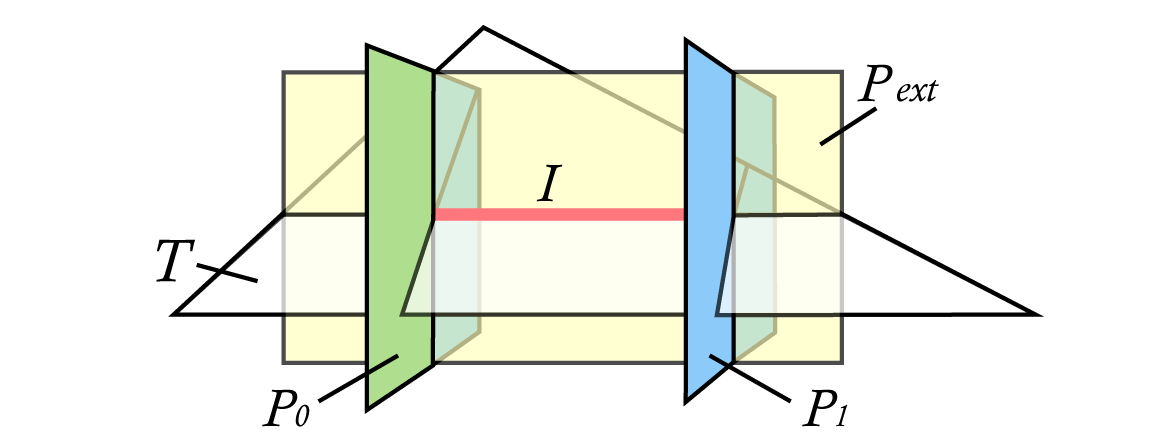
\includegraphics[width=3in]{boolean-13}
\caption{The geometry of planes in a PBI-rep. The red line segment ($\bm{\mathcal{I}}$) is the intersection represented by $\bm{\mathcal{I}}$.}
\label{fig:pbi}
\end{figure}

For example, two triangle faces, $t_1$ and $t_2$, originating from meshes $M_i$ and $M_j$ respectively, intersect. Two intersections are generated, ${\bm{\mathcal{I}}}_{12}$ on $t_1$ and ${\bm{\mathcal{I}}}_{21}$ on $t_2$.
For ${\bm{\mathcal{I}}}_{12}$, $T = t_1$ and $\bm{P}_{ext}=\bm{p}_{t_2, sp}$. $\bm{P}_0$ and $\bm{P}_1$ are boundary planes of $t_2$, which will be discussed later.
The last component $\mathcal{N}=t_2$ in general situation. Sometimes, ${\bm{\mathcal{I}}}_{12}$ may lie on the edge of $t_2$ (see Fig. \ref{fig:twin}). This is called \emph{edge intersection}. In this situation, the $\mathcal{N}$ is the set of all the faces from $M_j$ adjacent to that edge. Edge intersection is discussed in \S\ref{sec:degenerate}.


\subsubsection{Plane-based implementation}

\label{sec:embed}
\begin{figure}[t]
\centering
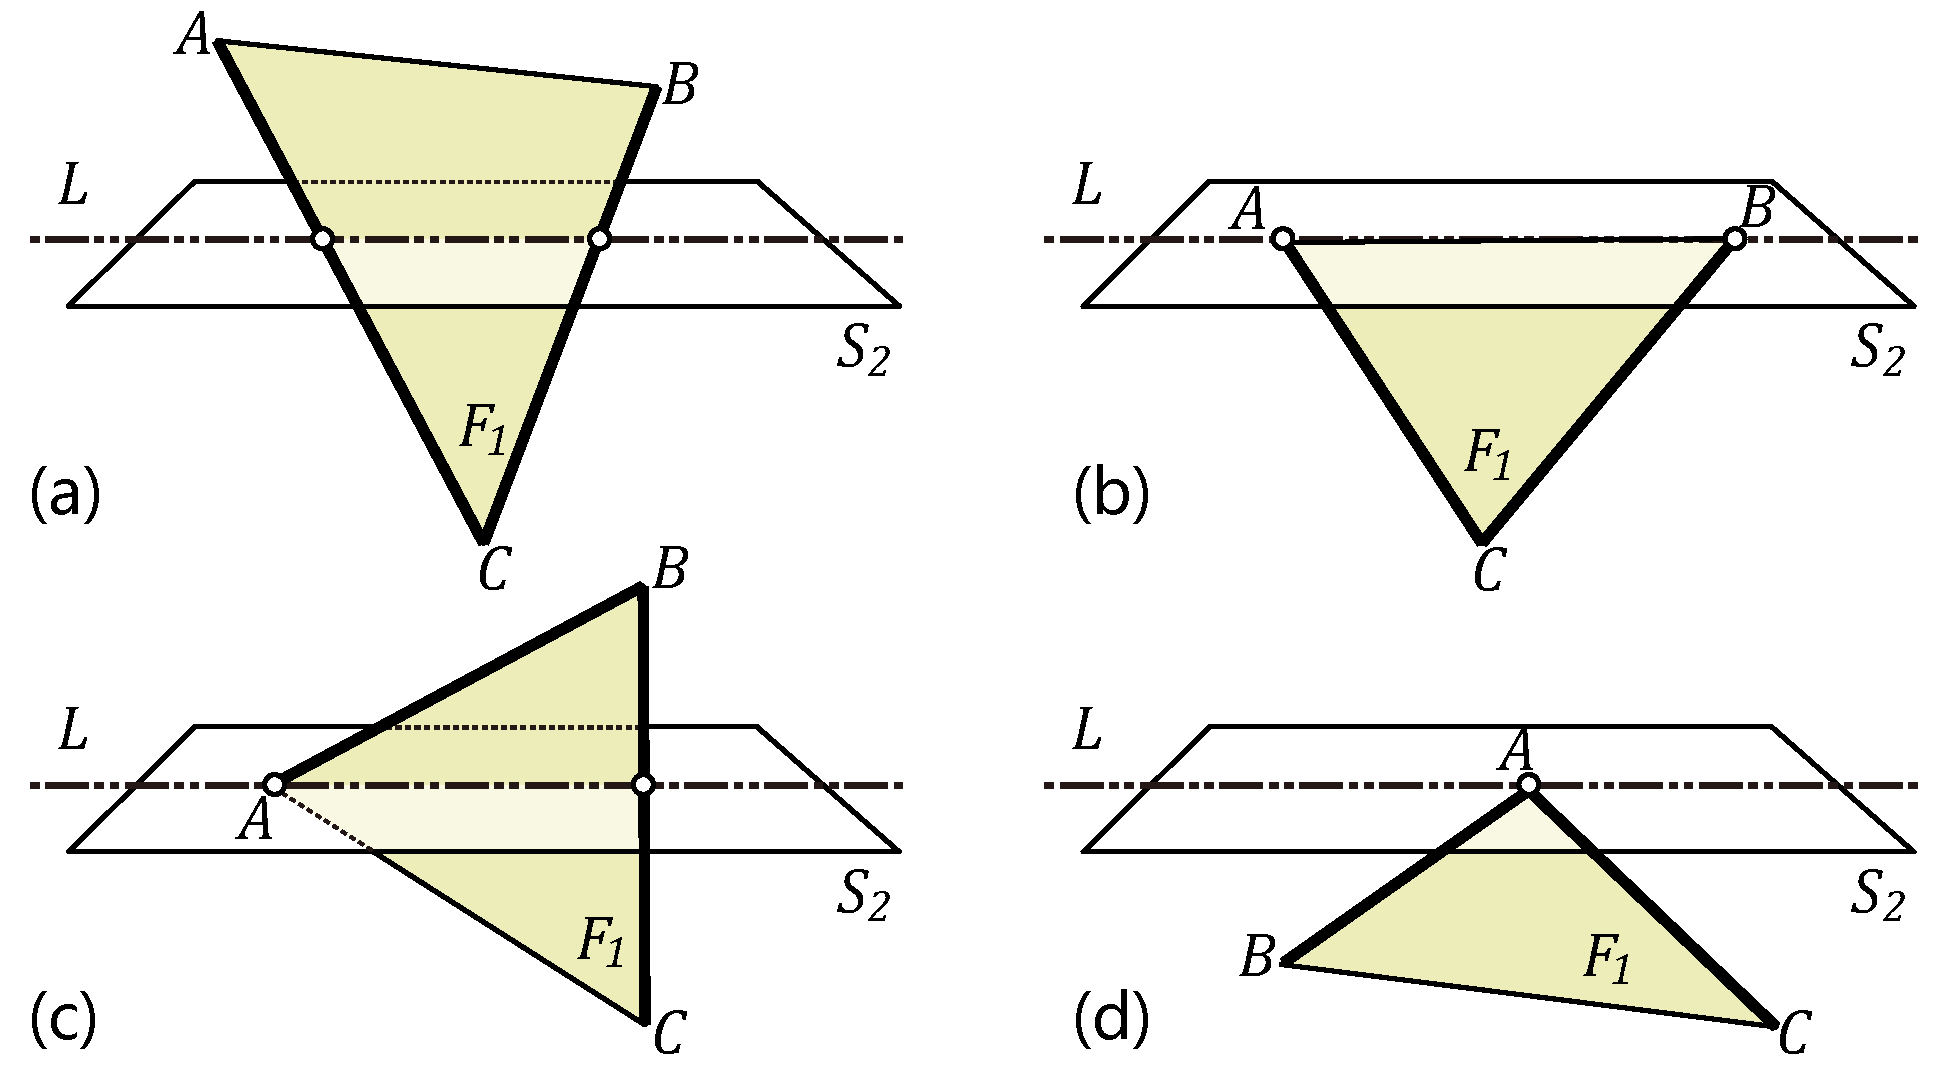
\includegraphics[width=3.5in]{sign}
\caption{We denote the signed distance from point $v_i$ to plane $\bm{p}_{t_2, sp}$ as $d_i$. The four conditions of intersection between $t_1$ and $\bm{p}_{t_2, sp}$ are:
(a) $d_0\cdot d_2<0$, $d_1\cdot d_2<0$;
(b) $d_0=0$, $d_1=0$, $d_2\neq 0$;
(c) $d_0=0$, $d_1\cdot d_2<0$;
(d) $d_0=0$, $d_1\cdot d_2>0$. End points of $Seg_1$ are the intersections between $\bm{p}_{t_2, sp}$ and the related edges of $t_1$ (bold red lines).}
\label{fig:isect}
\end{figure}

To implement M\"{o}ller's algorithm by plane-based geometry, we first convert each triangle to its P-reps: a supporting plane $\bm{p}_{t, sp}$  surrounded by three bounding planes $\{\bm{p}_{t, b}^i|\ i = 0,1,2\}$. The substrates of the intersection algorithms are point-plane orientation \cite{bernstein2009fast} and linear order of points (\S\ref{sec:substrates}), both of which can be implemented by plane-based geometry.

In the first step, the computation of signed distances involves only the vertices coordinates and the supporting planes of triangles. Therefore, if the early rejections occur, the bounding planes are not needed at all. In addition, according to the conversion method of Campen et al.\cite{campen2010exact}, the supporting plane is represented by four double-precision floating-point numbers. The precisions of the first three parameters and the last parameter are $L_a$ and $L_d$ respectively. They hold the relation $L_d = L_a + L + 1$, where $L$ is the precision of the coordinates of input vertices. This means we can compute the signed distance exactly within double-precision. With these two facts, our early rejection does not involve plane-based computation, thus is very efficient.

If early rejection is not triggered and $t_1$ and $t_2$ are not coplanar, $Seg_1$ and $Seg_2$ are computed. The end points are intersections between the supporting plane of one triangle and an edge of the other triangle. By computing the bounding planes, the end points can be implicitly represented by plane triples, $\bm{p}_{t_2, sp} \cap \bm{p}_{t_1, sp} \cap \bm{p}^i_{t_1, b}$, where $\bm{p}^i_{t_1, b}$ is the bounding plane of the related edge.
Fig. \ref{fig:isect} shows all of the possible intersection conditions between $t_1$ and $\bm{p}_{t_2, sp}$. The coplanar situation is discussed specifically in \S \ref{sec:degenerate}.

To avoid repetitive vertices in the final result, we perform vertex repetition elimination in this step. Because P-reps are used, the coincidence tests of the vertices are exact.



\subsection{Handling Degenerate Situations }
\label{sec:degenerate}

In most situations, intersections between triangles are line segments. However, they can also intersect on a point or a convex area. Even if the intersection is a line segment, the intersection can be on a primitive edge. These degenerate situations prevent us from performing robust boolean operations. In this section, we demonstrate our simple but effective ways of dealing with these degenerations, which conceals the complexity of intersections, and simplifies later processing.


\subsubsection{Point intersection}
\label{sec:ipoint}

If two triangles intersect at a single point (e.g., Fig. \ref{fig:isect}d) then the intersection cannot be represented using our PBI-rep. In this situation, we simply add the intersection point into the related triangles, guaranteeing correct tessellation. No intersection line segment is introduced.

\subsubsection{Edge intersection}


When a triangle intersects with the edge of other triangle, the generated intersection is referred as \emph{edge intersection}. The neighboring faces of the intersection is the set of all the faces that shared the edge rather than a single face. For example, in Fig. \ref{fig:twin}a, the neighboring faces of the intersection on $t_1$ are $t_2$ and $t^*_2$. The same intersection on $t_1$ will be detected twice, because $t_1$ intersects both $t_2$ and $t_2^*$ at the same line segment. In fact, edge intersections are often detected for multiple times. We solve this duplication in tessellation stage (see \S\ref{sec:tessellation}). We regard $t_2$ and $t_2^*$ as \emph{companion} triangles, because they are the neighboring faces of the same edge intersection. This concept will be referred to again in the discussion of coplanar cases.

\begin{figure}[t]
\centering
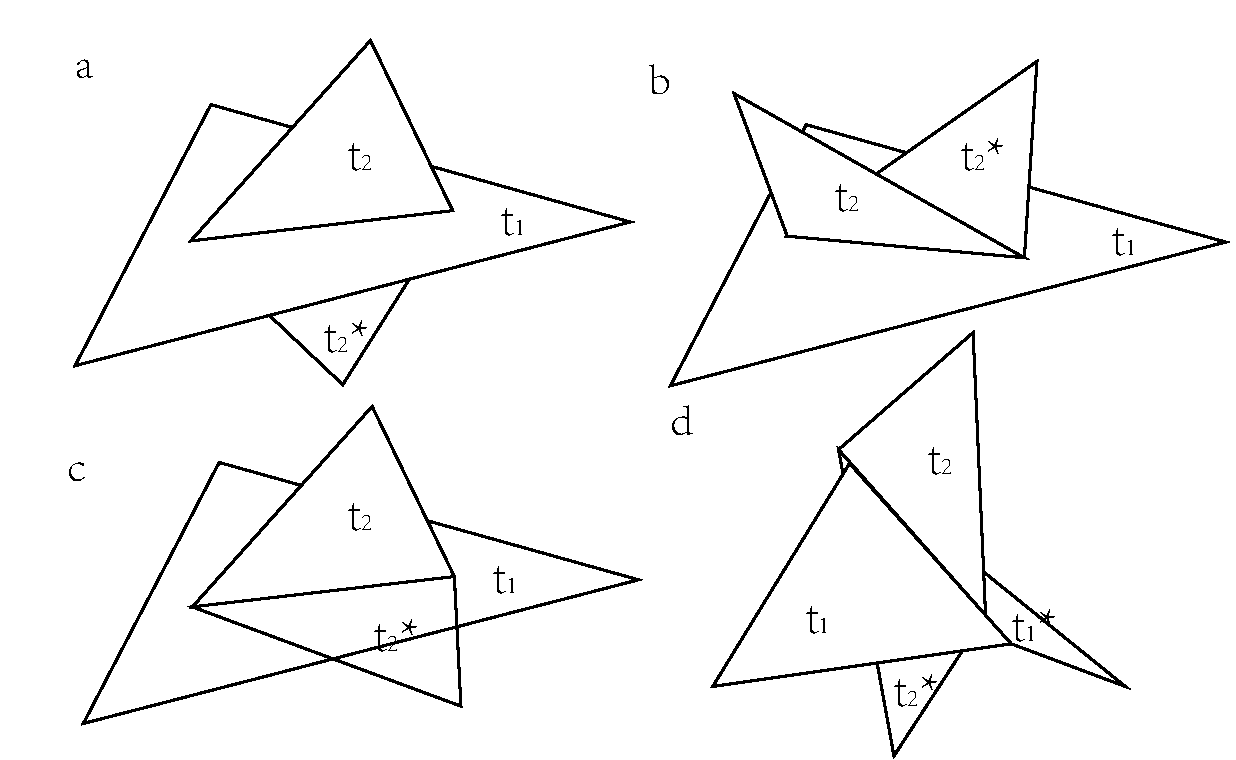
\includegraphics[width=3.5in]{edgeisect}
\caption{Different conditions of edge intersection. Triangle faces $t_1$ and $t_1^*$ are companion faces. Triangle faces $t_2$ and $t_2^*$ are companion faces. a) $t_2$ and $t_2^*$ are on different sides of $t_1$. b) $t_2$ and $t_2^*$ are on the same side of $t_1$. c) $t_2^*$ is coplanar with $t_1$. d) Both $t_1$ and $t_2$ have companion faces: the intersection is an edge intersection for both $t_1$ and $t_2$ (instead of only for $t_2$ is the previous three conditions). }
%Different conditions of edge intersection.
\label{fig:twin}
\end{figure}


\subsubsection{Copalnar}

\begin{figure}[t]
\centering
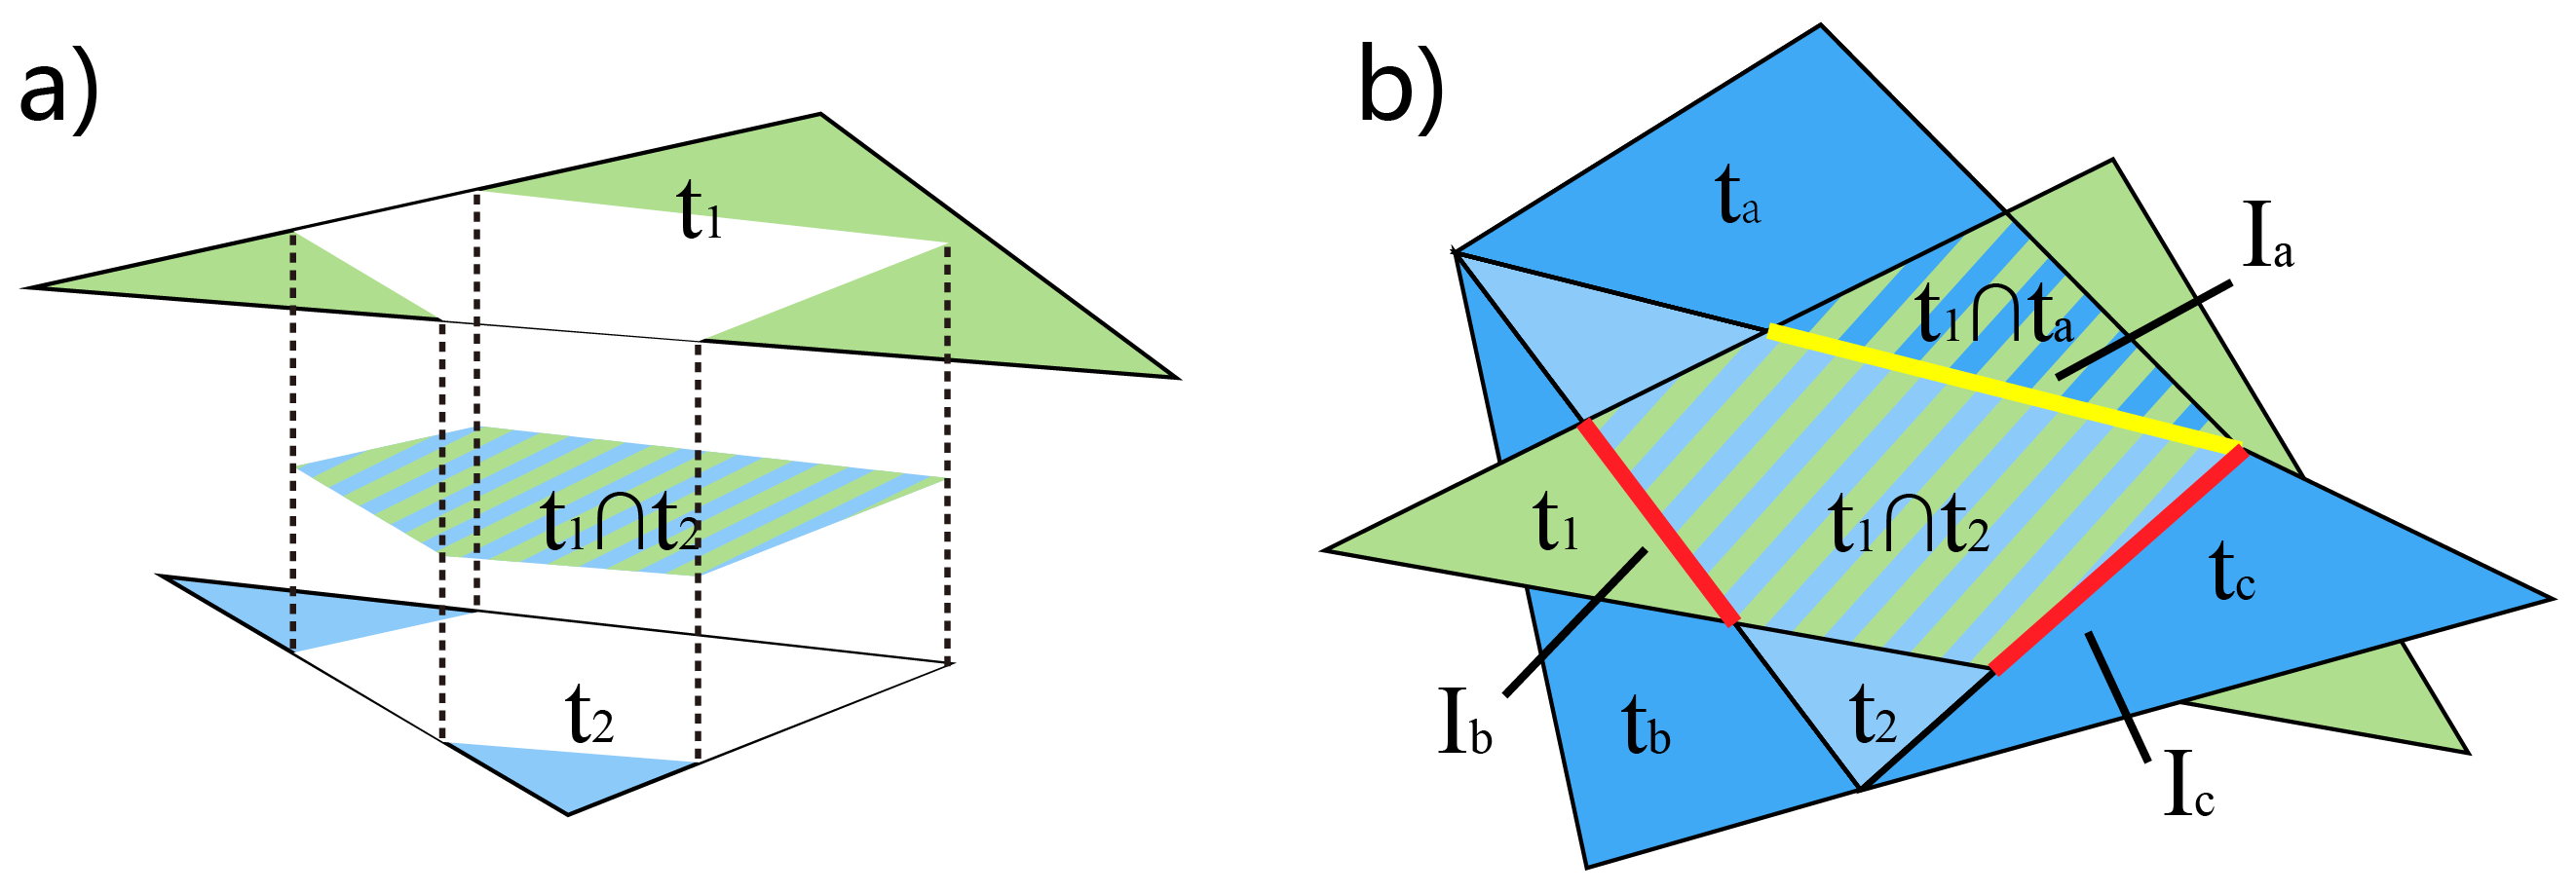
\includegraphics[width=3.5in]{boolean-03}
\caption{a) Coplanar situation. $t_1$ and $t_2$ intersect in 2D, dividing each other into a convex overlapping area and a exclusive area. b) Possible configurations of the companion faces. The blue triangles originate from the same mesh. For the yellow segment, it is not necessary in the final mesh, and it will not be detected. For the red segments, the companion triangles are not coplanar with $t_1$, so they can be detected during intersection tests between $t_1$ and the companion triangles ($t_a$ and $t_b$).}
\label{fig:coplanar}
\end{figure}


Consider two triangle faces, $t_1$ and $t_2$, which intersect within a common plane. Both $t_1$ and $t_2$ divide each other into two areas--a convex overlapping area and a exclusive area (see Fig. \ref{fig:coplanar}a). If we tessellate both $t_1$ and $t_2$ according to the boundary of the overlapping area, we can guarantee correct topology. This strategy is adopted by many previous methods \cite{feito2013fast,zhou2016mesh}. Conversely, in our method, we treat coplanar situations as if they do not intersect at all. We do not need any 2D intersection test. In this way, we avoid the processing of complex situations of 2D intersections, while having no side effect on the topological correctness.

We find that $t_1$ is actually clipped by edges of $t_2$ (see \ref{fig:coplanar}b). That means that we can view 2D intersections as special cases of edge intersections. There can be up to three edge intersections in one 2D intersection (red and yellow line segments). As discussed, edge intersections will be detected for multiple times by the companion triangles. Hence, we can rely on them to detect the intersections.

However, if all the companion triangles are coplanar, none of them will detect the intersection (the yellow segment). Fortunately, the intersection is not necessary in this situation. The neighboring faces of the intersection are all within the same plane. If such intersection is on the surface of the final mesh, the surface in the neighborhood of this intersection must be a plane. Therefore, the intersection is not necessary to be an edge in the final model and we can omit it.

Because we do not process coplanar intersections, the coplanar areas (the stripe areas) may have different tessellations in different primitives. It seems that inconsistent topology can occur in the final mesh. In fact, we do not need to worry about that, because faces from a certain primitive in such coplanar area are collected or abandoned together. The coplanar area, if on the surface of the final mesh, will inherit only one of the tessellations.
